\documentclass[12pt,a4paper]{ctexart}

% ---- 页面设置 ----
\usepackage[top=2.5cm, bottom=2.5cm, left=2.5cm, right=2.5cm]{geometry}
\usepackage{graphicx}
\graphicspath{{../../项目图片/}}
\usepackage{hyperref}
\usepackage{listings}
\usepackage{xcolor}
\usepackage{enumitem}
\usepackage{amsmath}
\usepackage{tikz}
\usetikzlibrary{positioning}
\usepackage{float}
\usepackage{tabularx}
\usepackage{booktabs}
\usepackage{fancyhdr}
\usepackage{titlesec}

\hypersetup{
    colorlinks=true,
    linkcolor=blue,
    urlcolor=cyan,
    citecolor=green
}

\definecolor{codebg}{RGB}{245,245,245}
\definecolor{codeframe}{RGB}{200,200,200}

\lstset{
    basicstyle=\ttfamily\small,
    backgroundcolor=\color{codebg},
    frame=single,
    rulecolor=\color{codeframe},
    breaklines=true,
    numbers=left,
    numberstyle=\tiny\color{gray},
    tabsize=2,
    language=C
}

\pagestyle{fancy}
\setlength{\headheight}{14pt}
\fancyhf{}
\fancyhead[L]{\small 智能交互终端技术报告}
\fancyhead[R]{\small STM32F407 + ASR PRO + ESP8266}
\fancyfoot[C]{\thepage}
\renewcommand{\headrulewidth}{0.5pt}

\title{\textbf{智能交互终端技术报告}\\
       \large 基于 STM32F407 的多模态智能交互终端}
\author{}
\date{2026年8月}

\begin{document}

\maketitle
\thispagestyle{empty}

\begin{center}
\begin{tabular}{rl}
\textbf{项目名称} & 智能交互终端 \\
\textbf{主控芯片} & STM32F407VET6 (ARM Cortex-M4, 168MHz) \\
\textbf{语音识别} & 天问 ASR PRO (CI-03T 离线语音芯片) \\
\textbf{WiFi通信}   & ESP8266 (ESP-AT 固件, 802.11 b/g/n) \\
\textbf{显示屏}     & 2.8寸 TFT-LCD (240×320, ILI9341, 16位并口) \\
\textbf{触摸屏}     & GT9147 电容触摸 (I2C) \\
\textbf{环境传感器} & AHT20 温湿度 + BMP280 气压/海拔 (I2C) \\
\textbf{操作系统}   & FreeRTOS (CMSIS-RTOS v2) \\
\textbf{图形库}     & LVGL v8.3 \\
\textbf{云端AI}     & 阿里云 DashScope (Qwen 3.8-Max) \\
\textbf{开发环境}   & STM32CubeMX + Keil MDK-ARM \\
\end{tabular}
\end{center}

\vspace{1cm}

\begin{abstract}
\noindent 本项目设计并实现了一款智能交互终端。系统以 STM32F407 为主控制器，集成 LVGL 图形界面、虚拟表情动画、ASR PRO 离线语音命令控制、模拟时钟、日历、环境数据采集，以及通过 ESP8266 连接阿里云 DashScope 大模型实现的云端 AI 对话功能。系统采用 FreeRTOS 多任务架构，通过消息队列实现模块间解耦通信，支持触摸屏拼音输入、离线语音命令、WiFi 扫描选择和串口/WiFi IAP 固件升级，实现了较完整的嵌入式智能交互闭环。
\end{abstract}

\newpage
\tableofcontents
\newpage

% ============================================================
\section{系统总体架构}
% ============================================================

\subsection{硬件架构}

系统硬件由主控、语音、联网、显示触摸和环境传感器模块组成，通过串口、并行总线与 I2C 总线互联：

\begin{figure}[H]
\centering
\begin{tikzpicture}[node distance=2cm, auto]
    \tikzstyle{block} = [rectangle, draw, fill=blue!10, text width=3.5cm, text centered, rounded corners, minimum height=2cm]
    \tikzstyle{arrow} = [thick,->,>=stealth]

    \node [block] (stm32) {STM32F407VET6\\主控制器\\168MHz Cortex-M4};
    \node [block, above right=0.5cm and 2cm of stm32] (asr) {ASR PRO\\离线语音芯片\\CI-03T};
    \node [block, below right=0.5cm and 2cm of stm32] (esp) {ESP8266\\WiFi模块\\ESP-AT固件};
    \node [block, below=2cm of stm32] (lcd) {TFT-LCD\\2.8'' 240×320\\ILI9341 + GT9147};
    \node [block, below left=0.5cm and 2cm of stm32] (sensor) {AHT20 + BMP280\\温湿度/气压/海拔\\I2C传感器};

    \draw [arrow] (asr) -- node[above] {USART1 115200} (stm32);
    \draw [arrow] (stm32) -- node[below] {USART3 115200} (esp);
    \draw [arrow] (stm32) -- node[left] {FSMC 16位并口} (lcd);
    \draw [arrow] (stm32) -- node[above,sloped] {I2C1} (lcd);
    \draw [arrow] (sensor) -- node[above,sloped] {I2C} (stm32);
\end{tikzpicture}
\caption{系统硬件拓扑}
\end{figure}

\subsection{软件架构}

系统基于 FreeRTOS 实现多任务并行调度，共 5 个核心任务：

\begin{table}[H]
\centering
\begin{tabularx}{\textwidth}{lXXl}
\toprule
\textbf{任务名} & \textbf{功能} & \textbf{优先级} & \textbf{栈大小} \\
\midrule
defaultTask & 系统初始化、外设自检 & Normal & 4KB \\
lvglTask & LVGL图形刷新、UI事件处理、表情动画、ASR命令处理 & AboveNormal & 16KB \\
esp8266Task & ESP8266 AT指令交互、WiFi连接、HTTP/HTTPS请求 & Normal & 4KB \\
asrTask & ASR PRO串口数据接收与解析 & Normal & 4KB \\
sensorTask & AHT20/BMP280 环境数据采集与上报 & Normal & 4KB \\
\bottomrule
\end{tabularx}
\caption{FreeRTOS 任务分配}
\end{table}

任务间通过 5 个消息队列通信：

\begin{itemize}
    \item \texttt{asr\_queue}：asrTask → lvglTask，传递语音命令 ID
    \item \texttt{esp\_ai\_req\_queue}：lvglTask → esp8266Task，传递 AI 对话请求
    \item \texttt{esp\_ai\_queue}：esp8266Task → lvglTask，传递 AI 回复文本
    \item \texttt{esp\_rx\_queue}：esp8266Task → lvglTask，传递系统状态日志
    \item \texttt{sensor\_queue}：sensorTask → lvglTask，传递温湿度、气压与海拔数据
\end{itemize}

% ============================================================
\section{用户界面设计}
% ============================================================

\subsection{页面结构}

系统包含 7 个 LVGL 页面，通过语音命令或触摸操作切换：

\begin{table}[H]
\centering
\begin{tabularx}{\textwidth}{llX}
\toprule
\textbf{页面} & \textbf{语音命令} & \textbf{功能描述} \\
\midrule
待机画面 (idle\_scr) & ``待机画面'' & 虚拟表情动画（眨眼、眼球游走） \\
主菜单 (main\_scr) & ``打开菜单'' & 4 个功能入口按钮，横向排列为桌面图标入口 \\
系统 (system\_scr)  & ``系统状态'' / ``设置'' & 可滚动系统日志、硬件信息、WiFi 设置入口 \\
WiFi (wifi\_scr) & 触摸进入 & 扫描周围热点、选择 SSID、输入密码并连接 \\
时钟 (clock\_scr)   & ``时钟'' & 模拟表盘时钟，包含 12 小时刻度与时分秒指针 \\
日历 (calendar\_scr) & ``日历'' & 月视图日历，支持前后翻月与当天高亮 \\
环境 (env\_scr) & 触摸进入 & 显示温度、湿度、气压和海拔数据 \\
AI对话 (ai\_scr)     & ``打开对话'' & 云端AI对话界面、拼音输入法 \\
\bottomrule
\end{tabularx}
\caption{UI 页面说明}
\end{table}

\subsection{界面展示}

\begin{figure}[H]
\centering
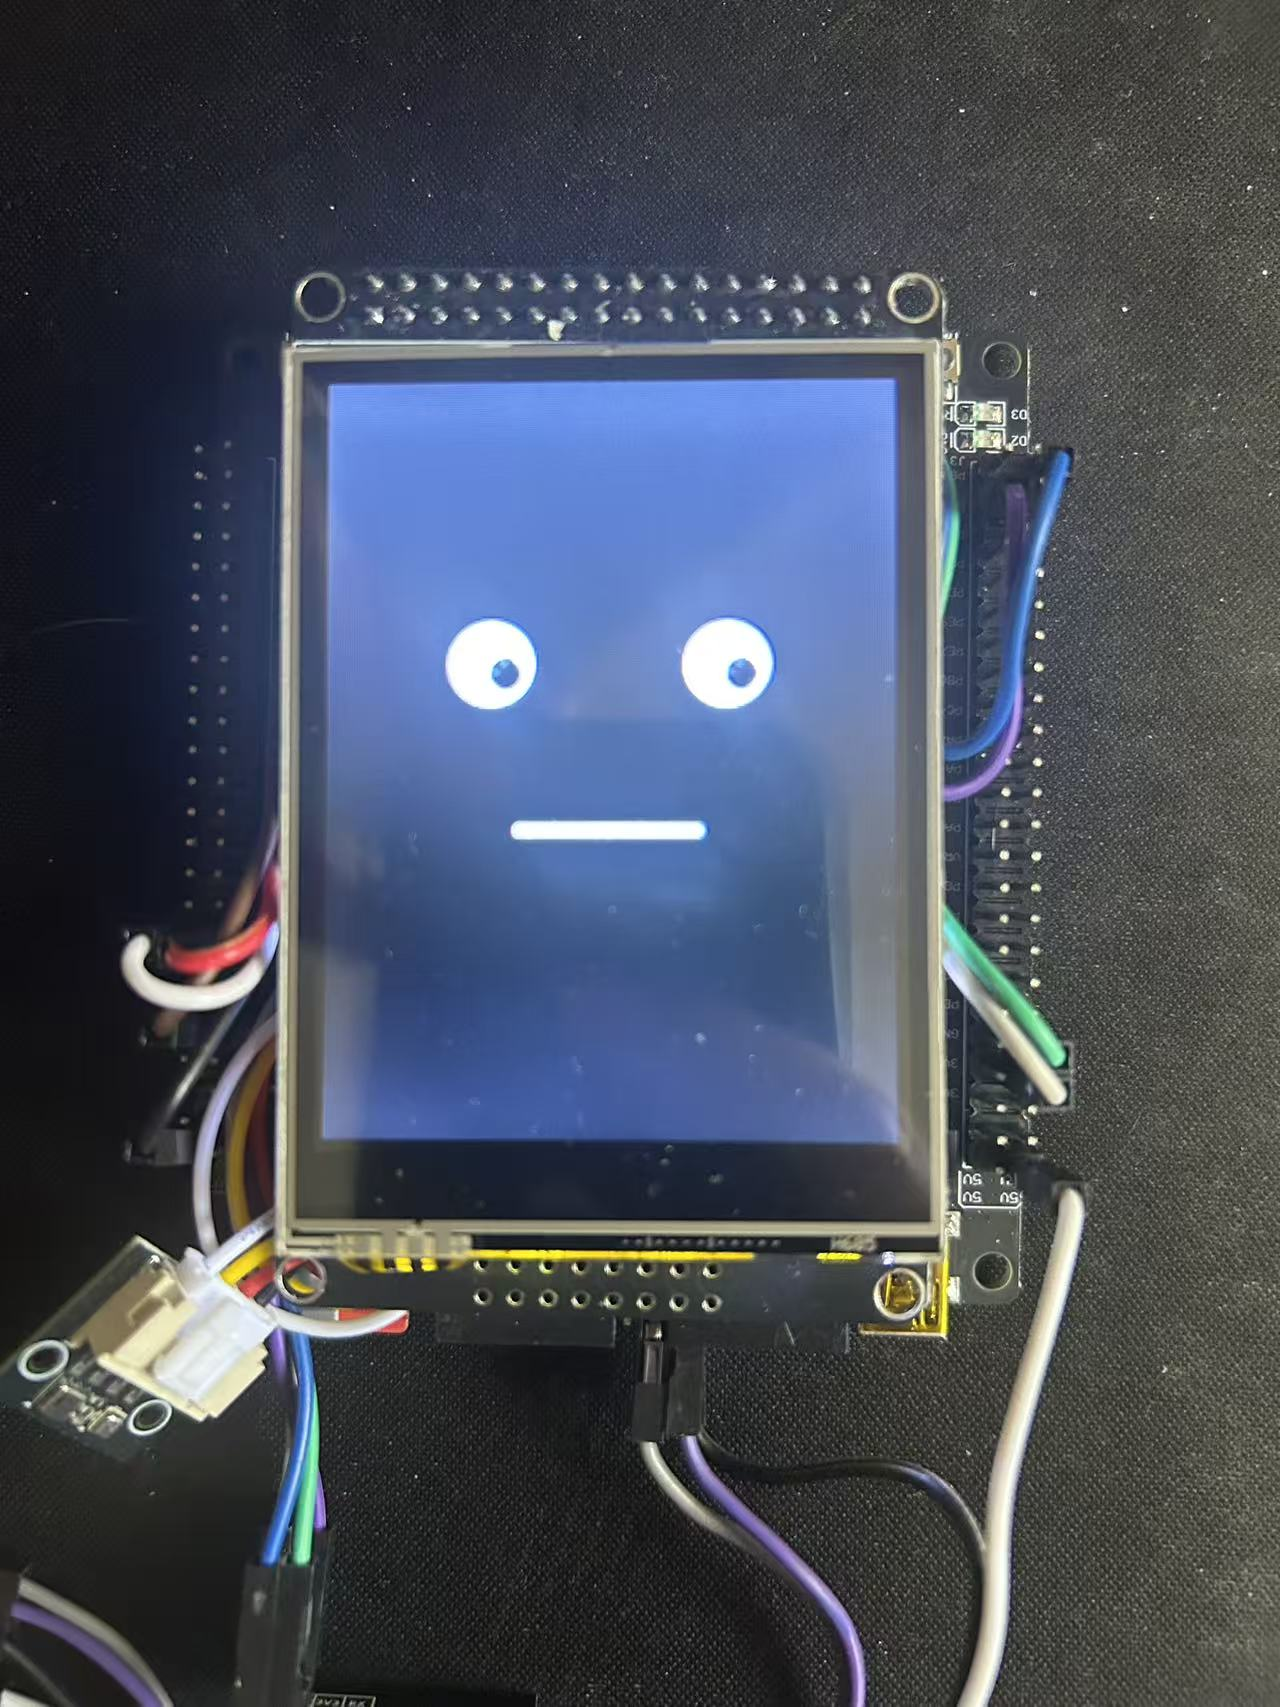
\includegraphics[width=0.32\textwidth]{表情.jpg}
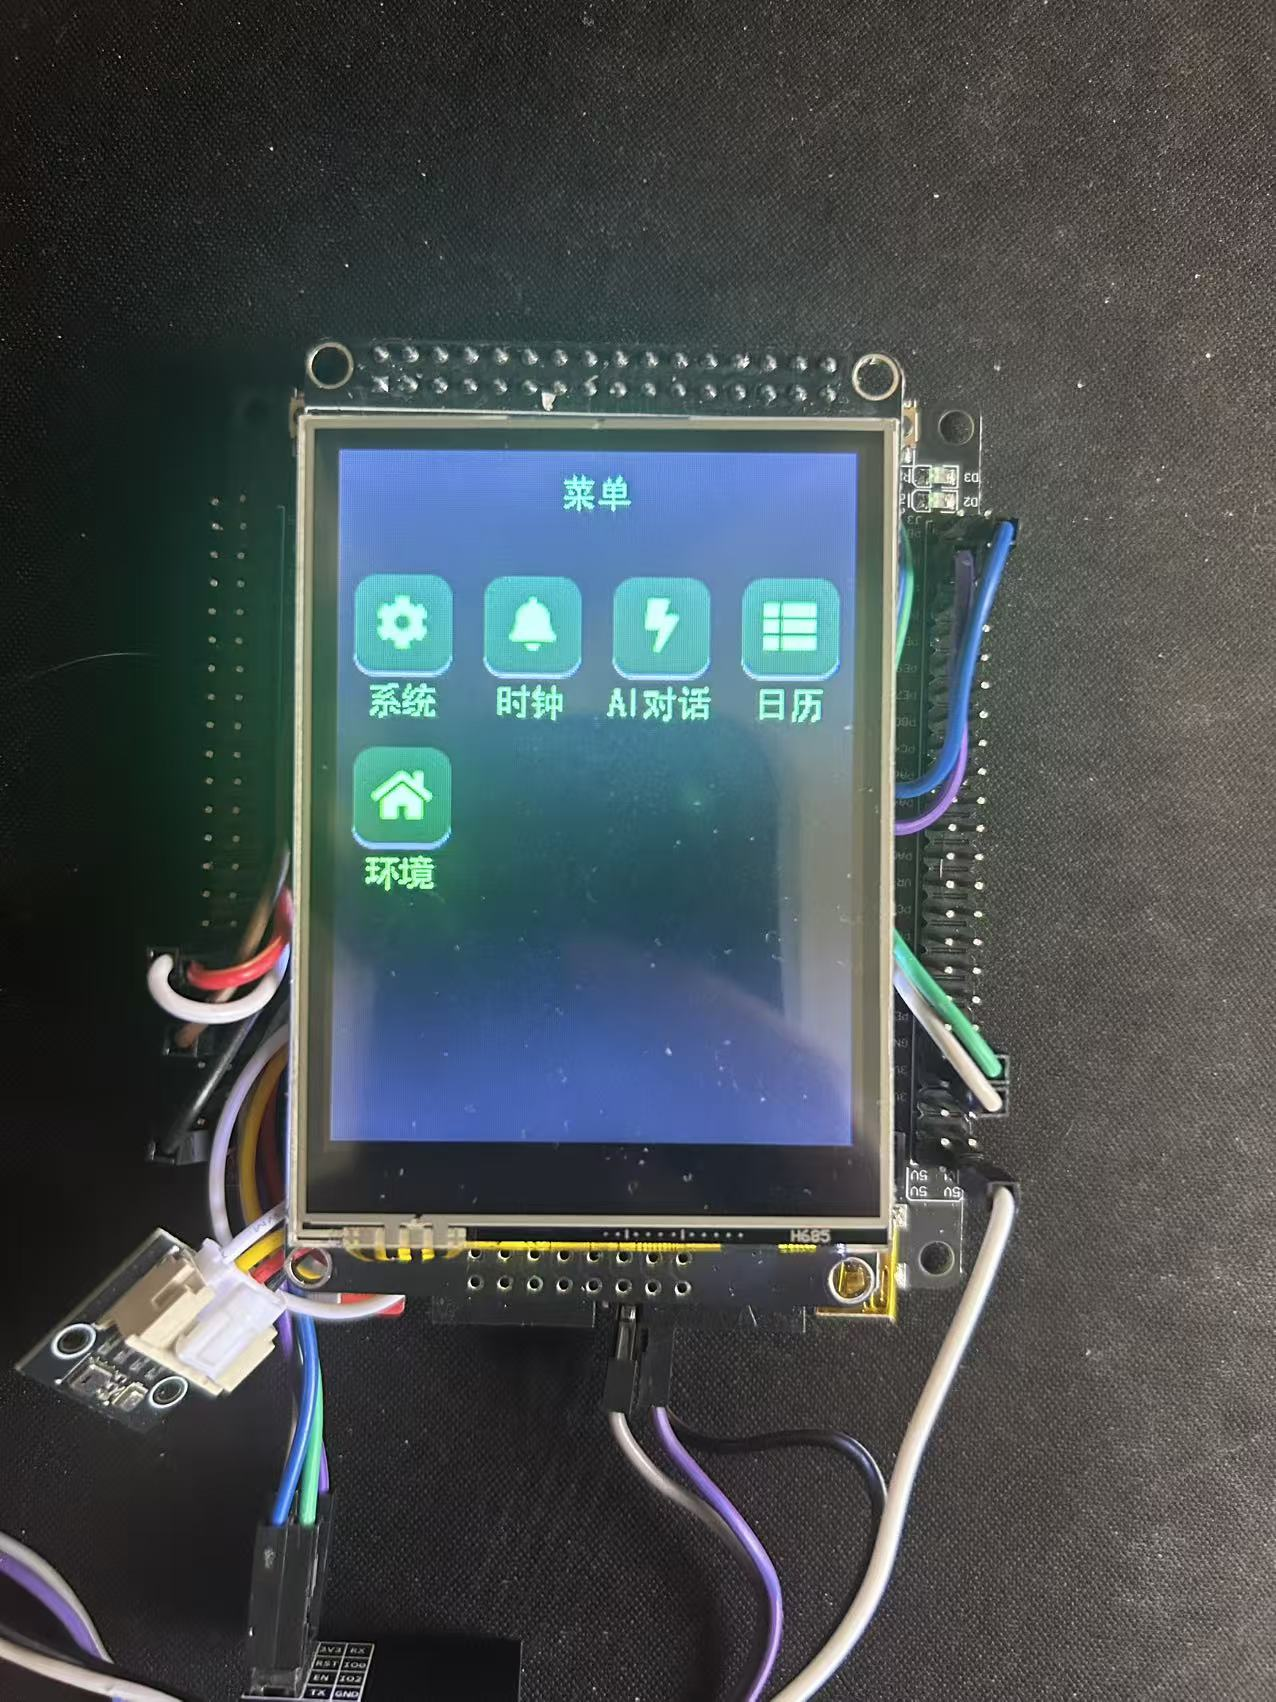
\includegraphics[width=0.32\textwidth]{菜单.jpg}
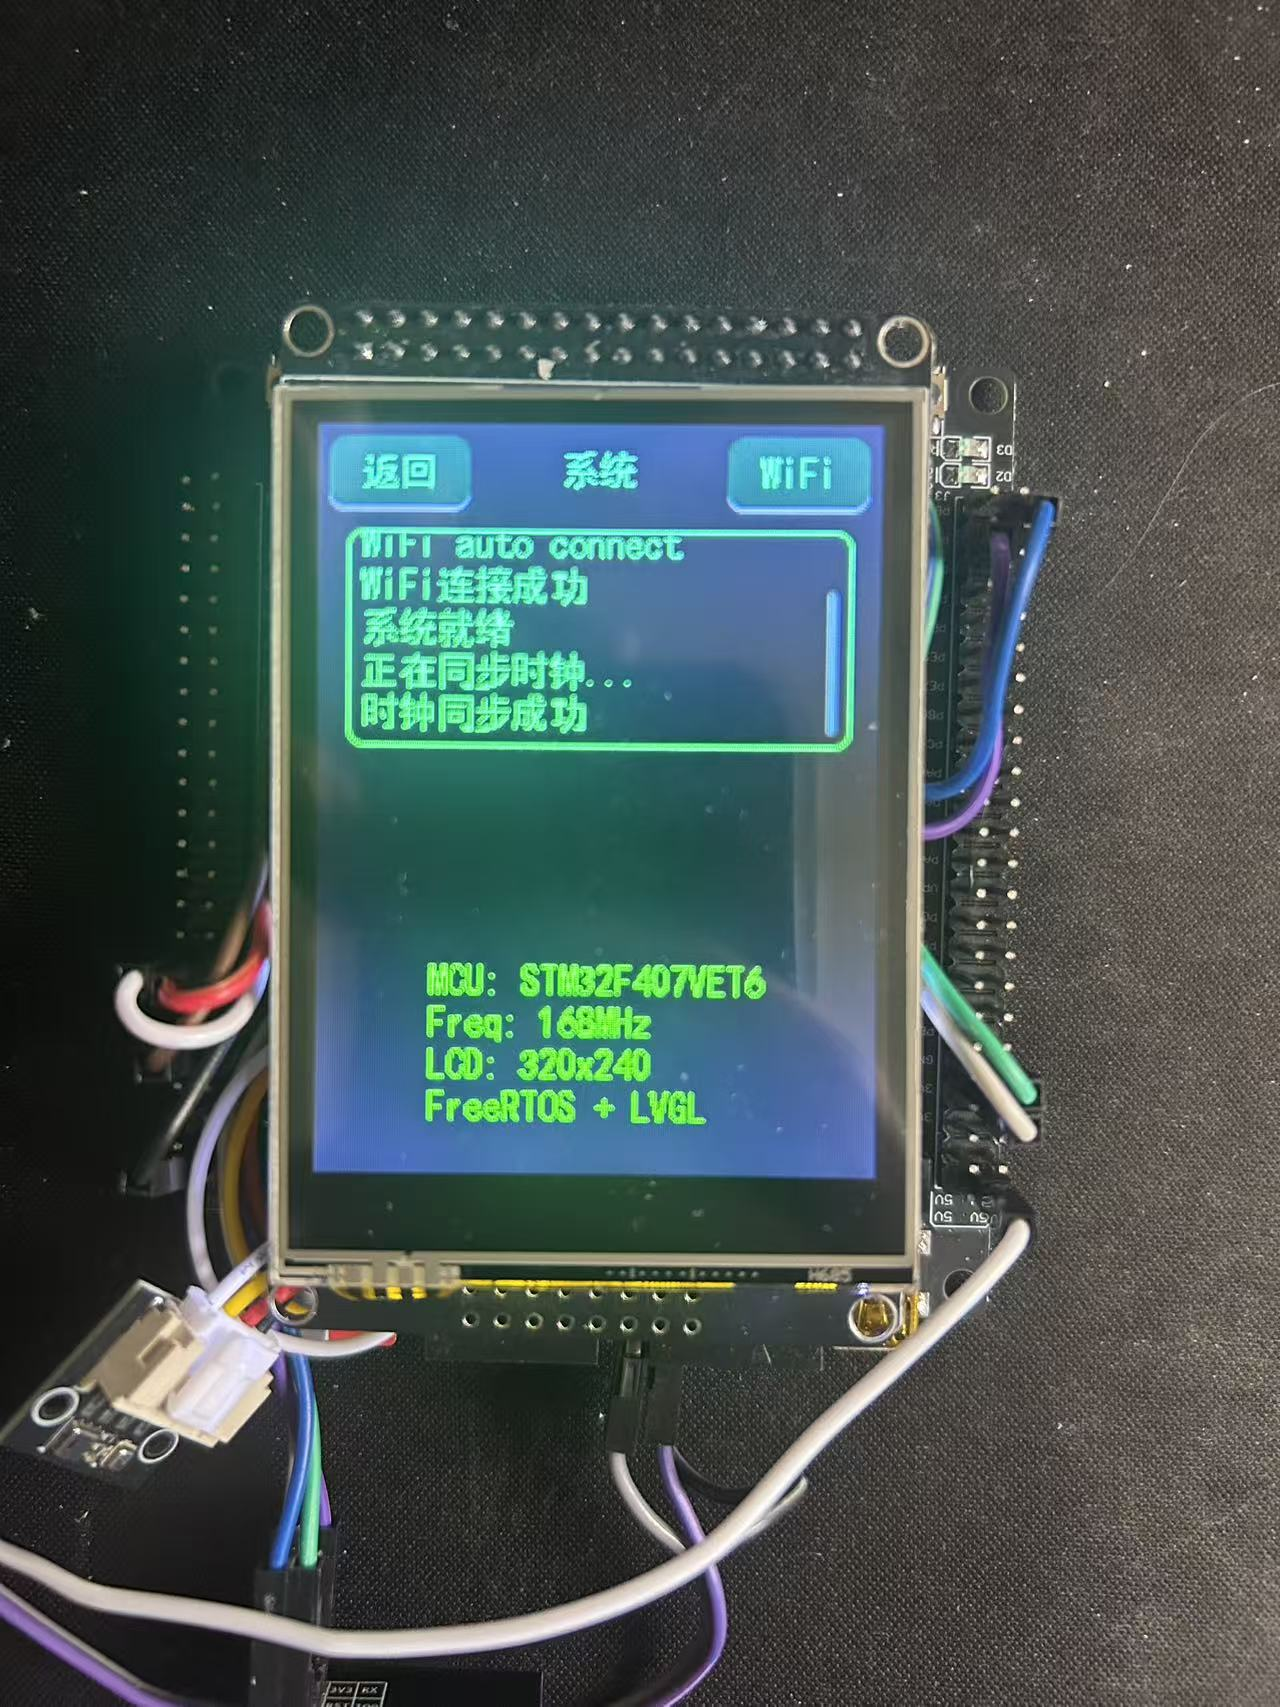
\includegraphics[width=0.32\textwidth]{系统界面.jpg}
\caption{待机表情、主菜单与系统日志界面}
\end{figure}

\begin{figure}[H]
\centering
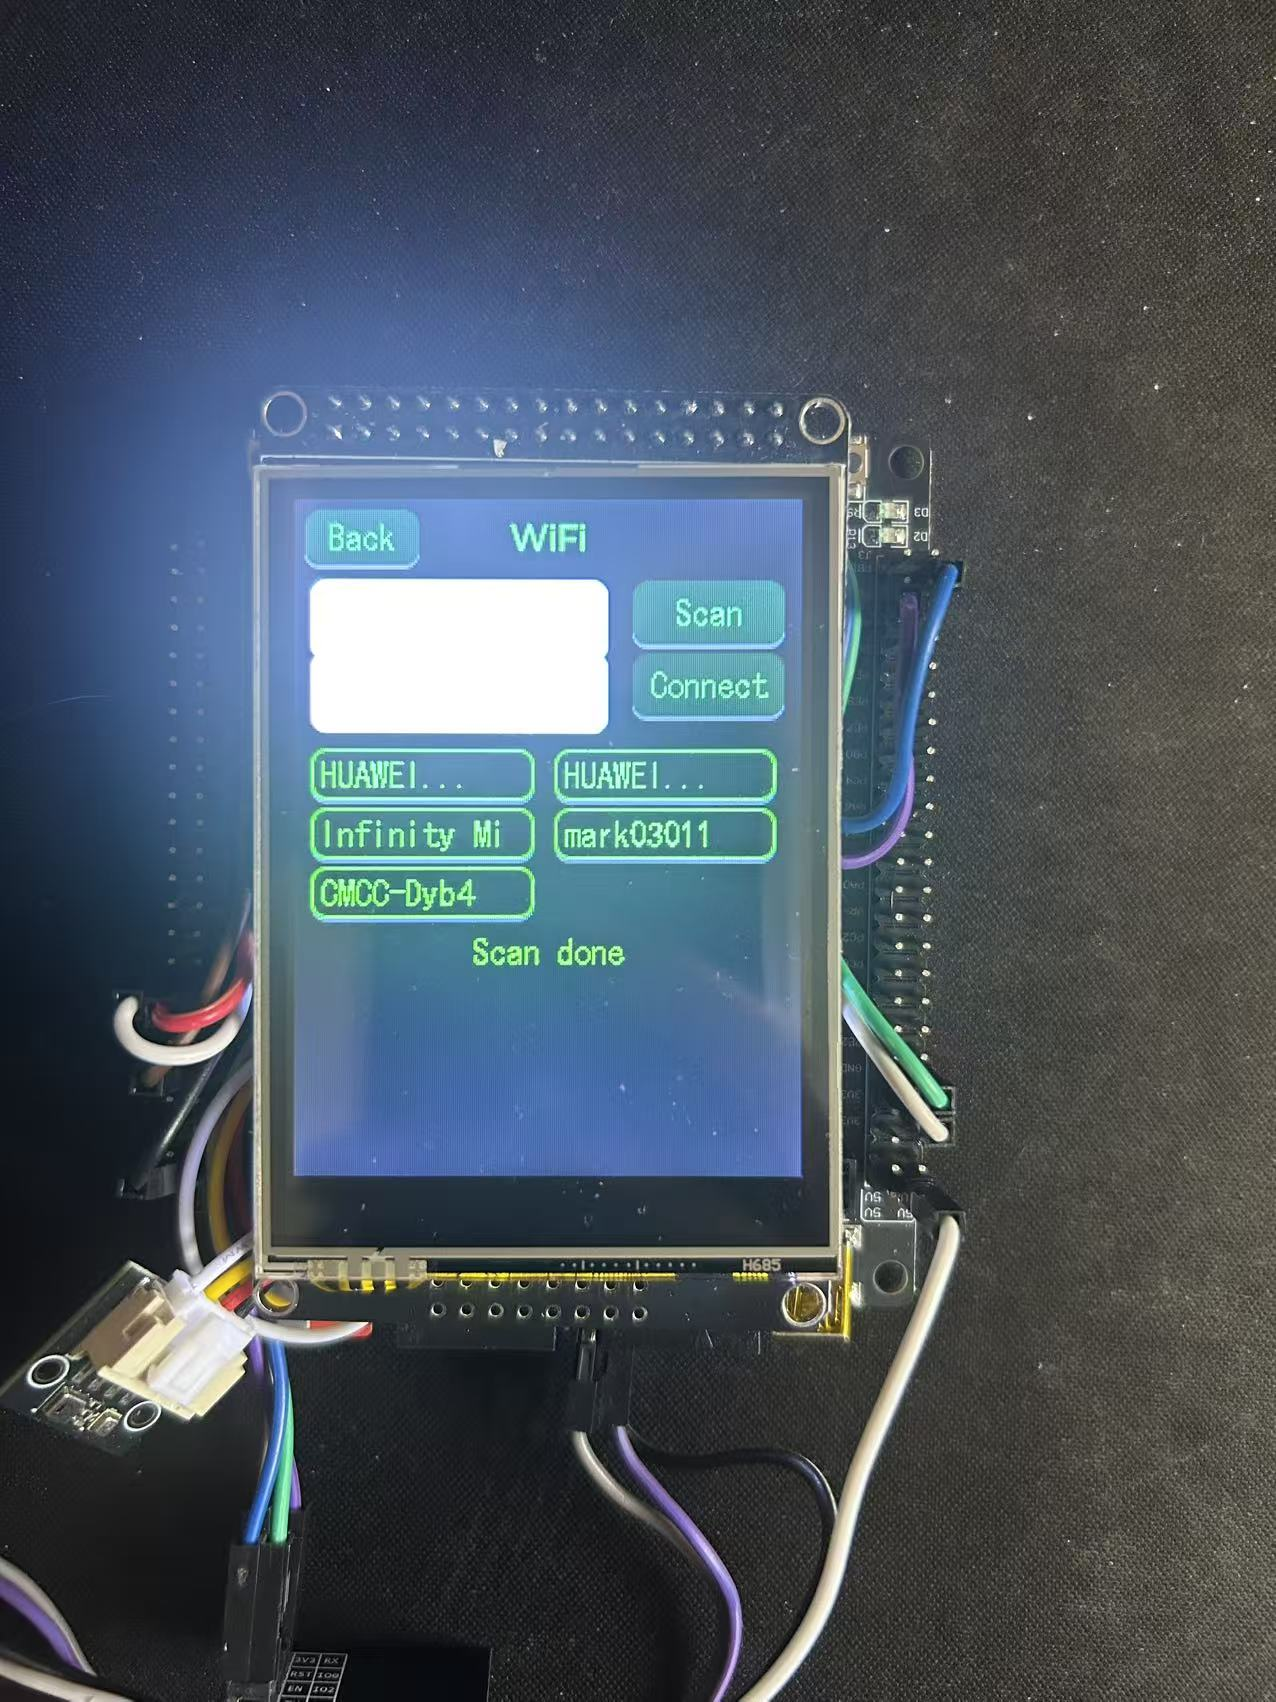
\includegraphics[width=0.32\textwidth]{wifi界面.jpg}
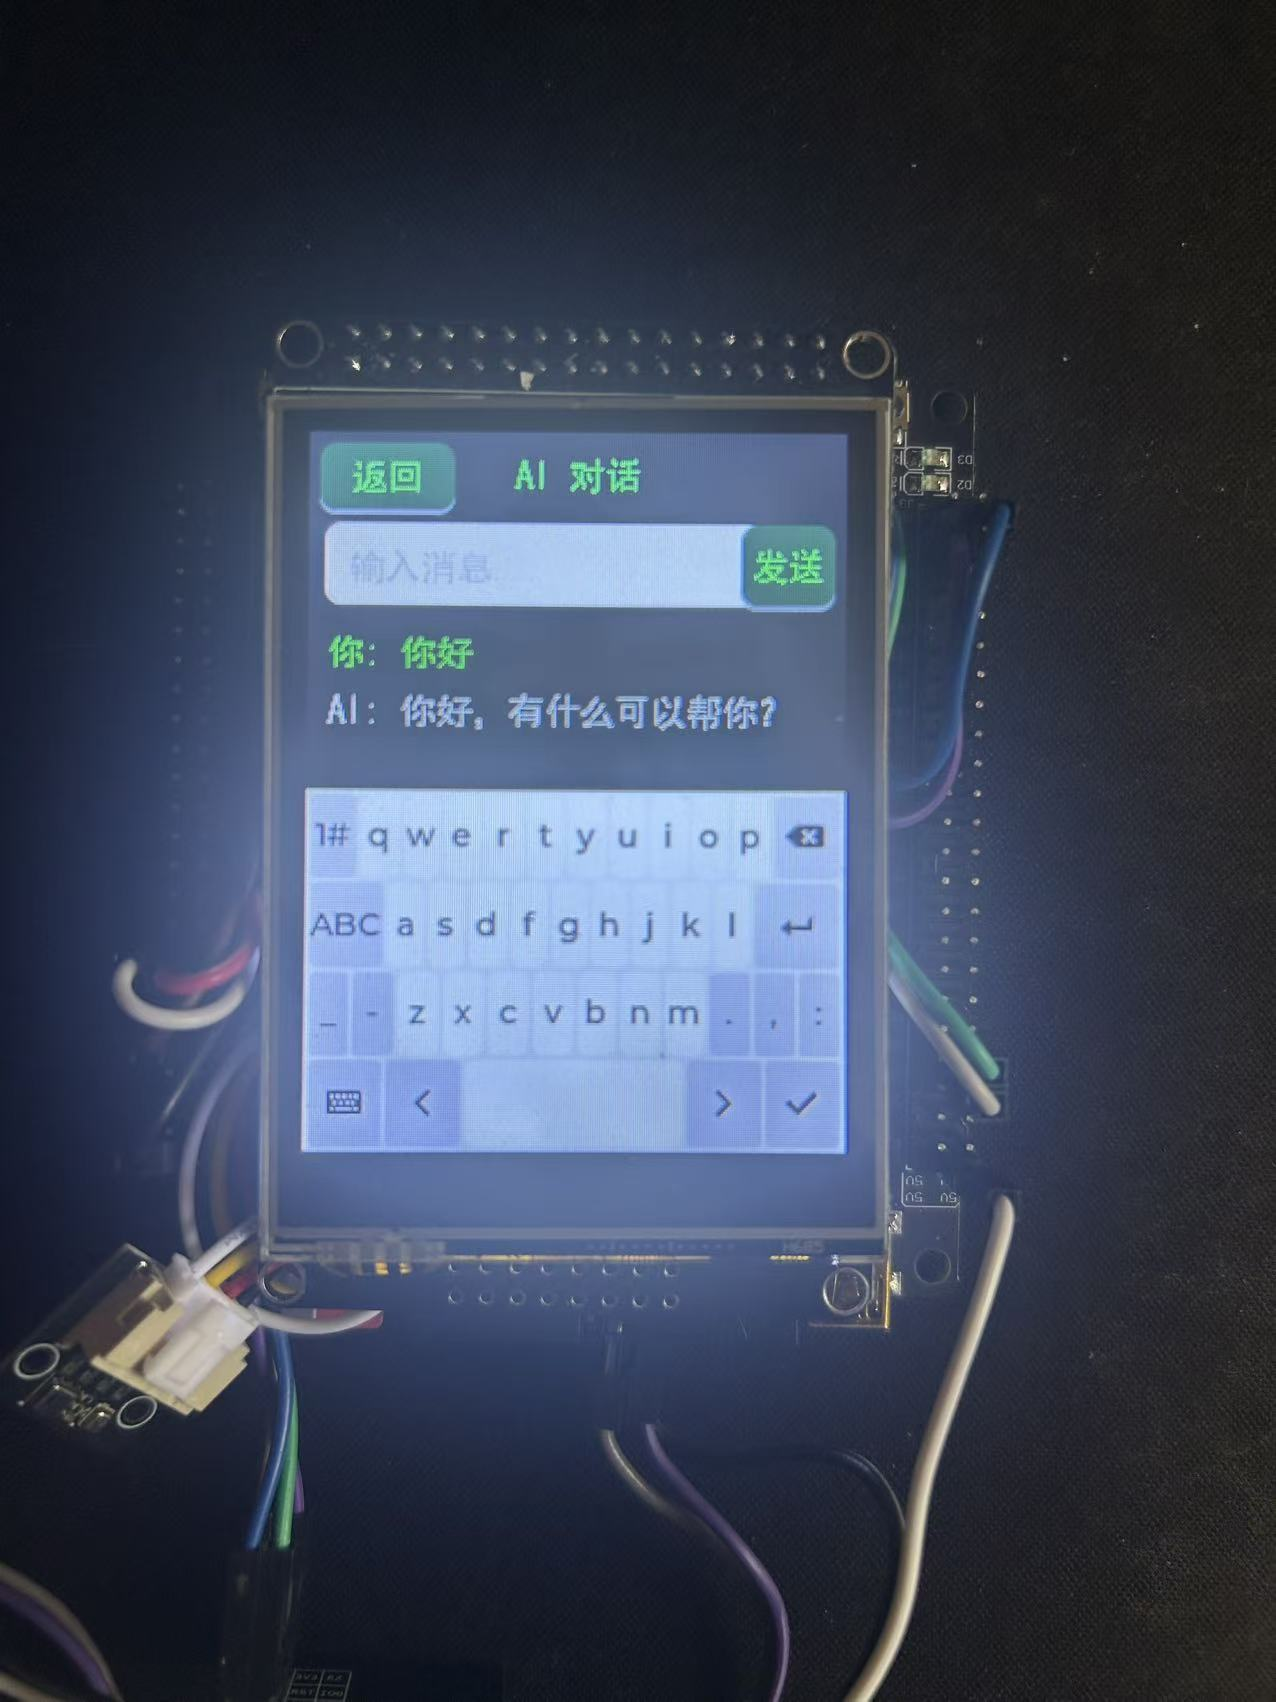
\includegraphics[width=0.32\textwidth]{ai对话.jpg}
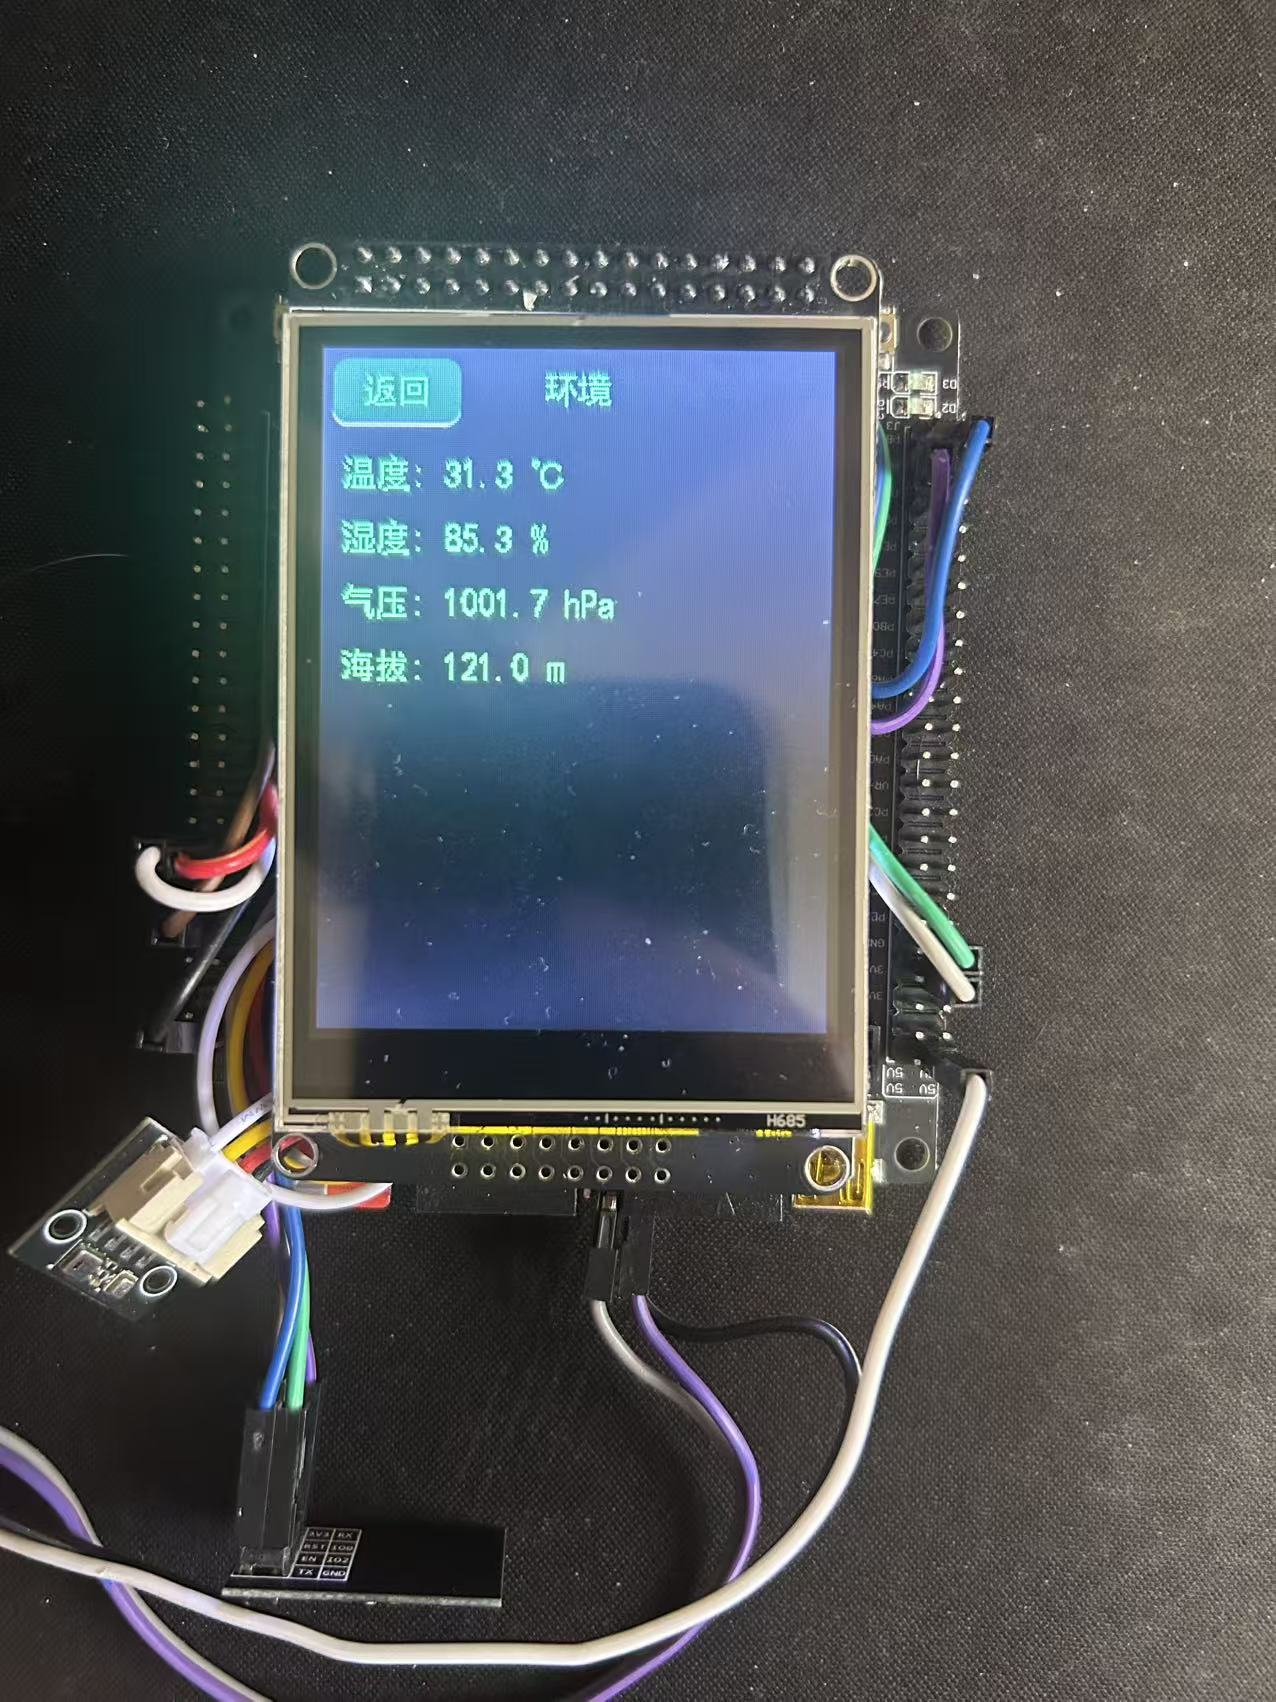
\includegraphics[width=0.32\textwidth]{环境.jpg}
\caption{WiFi 选择、AI 对话与环境监测界面}
\end{figure}

\begin{figure}[H]
\centering
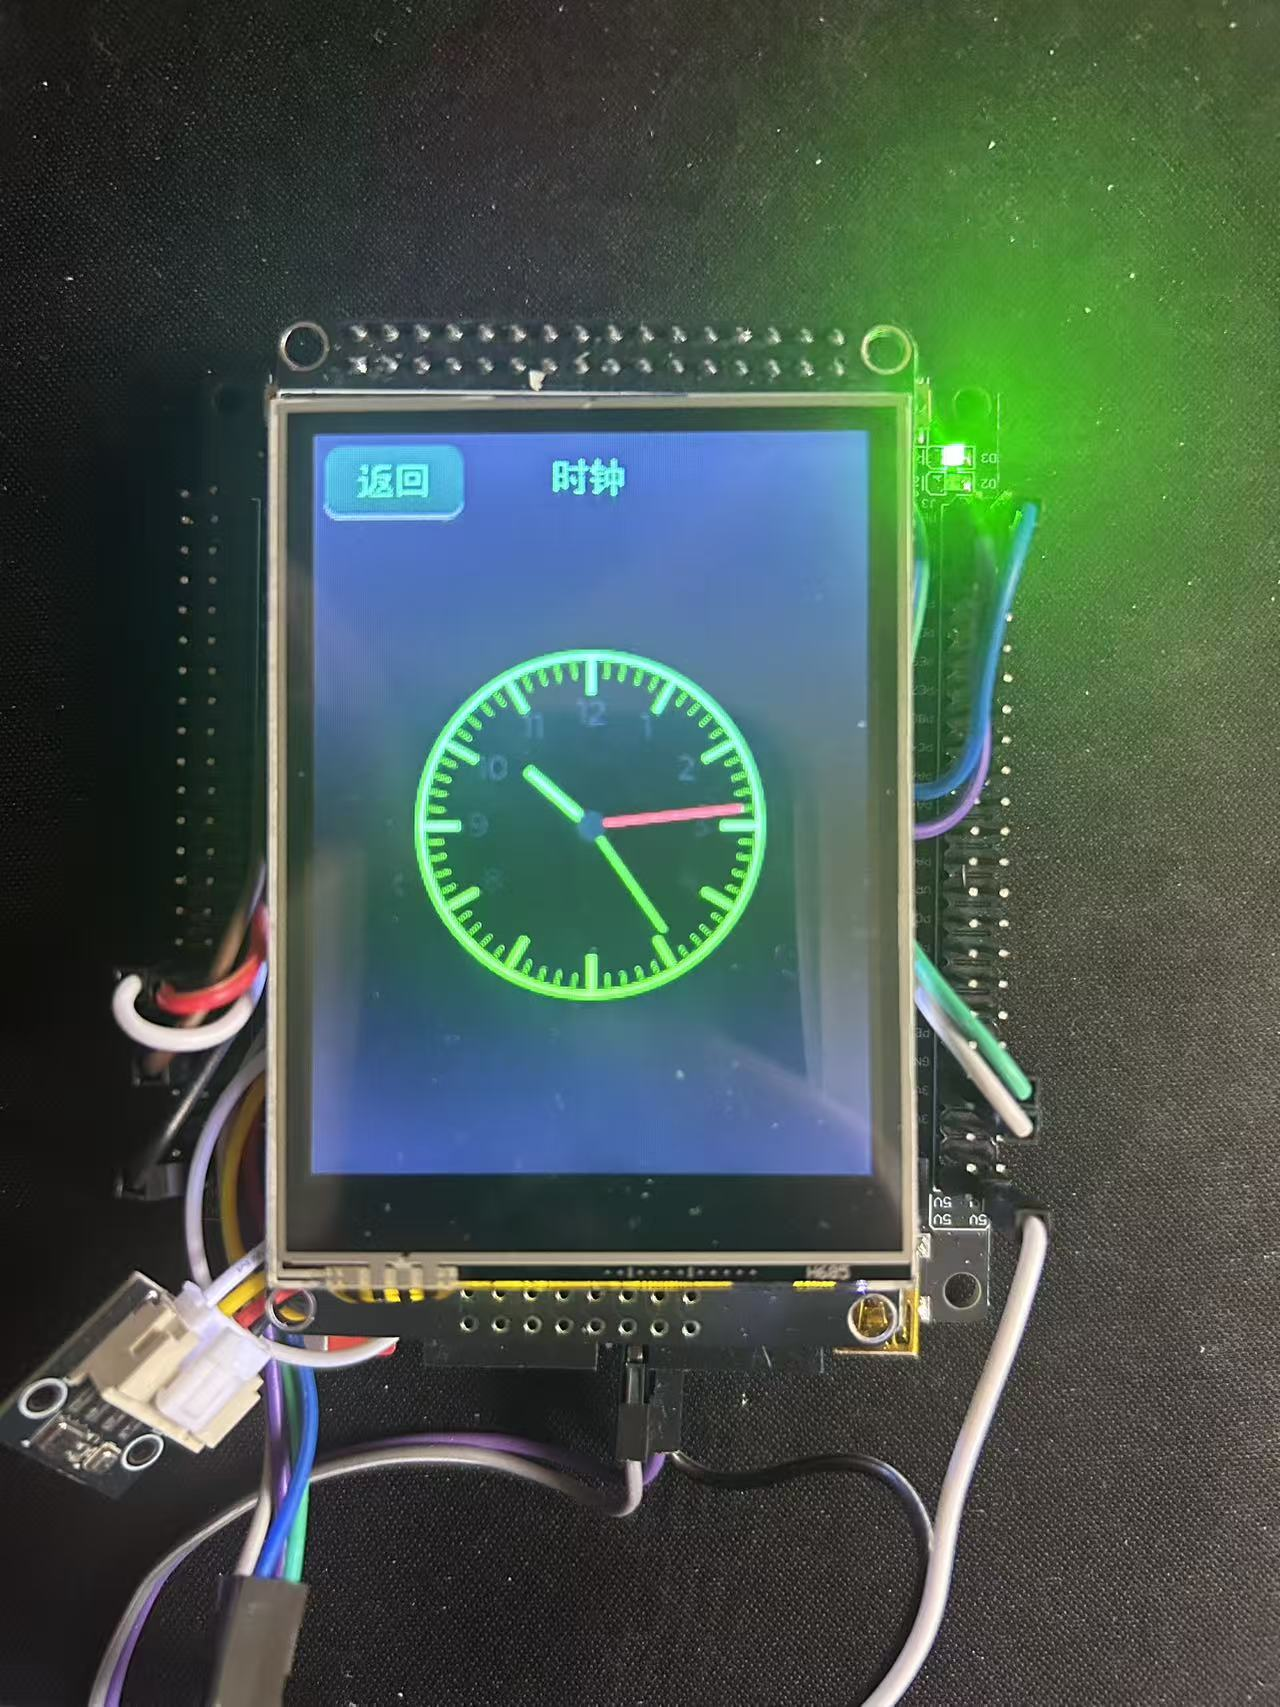
\includegraphics[width=0.42\textwidth]{时钟.jpg}
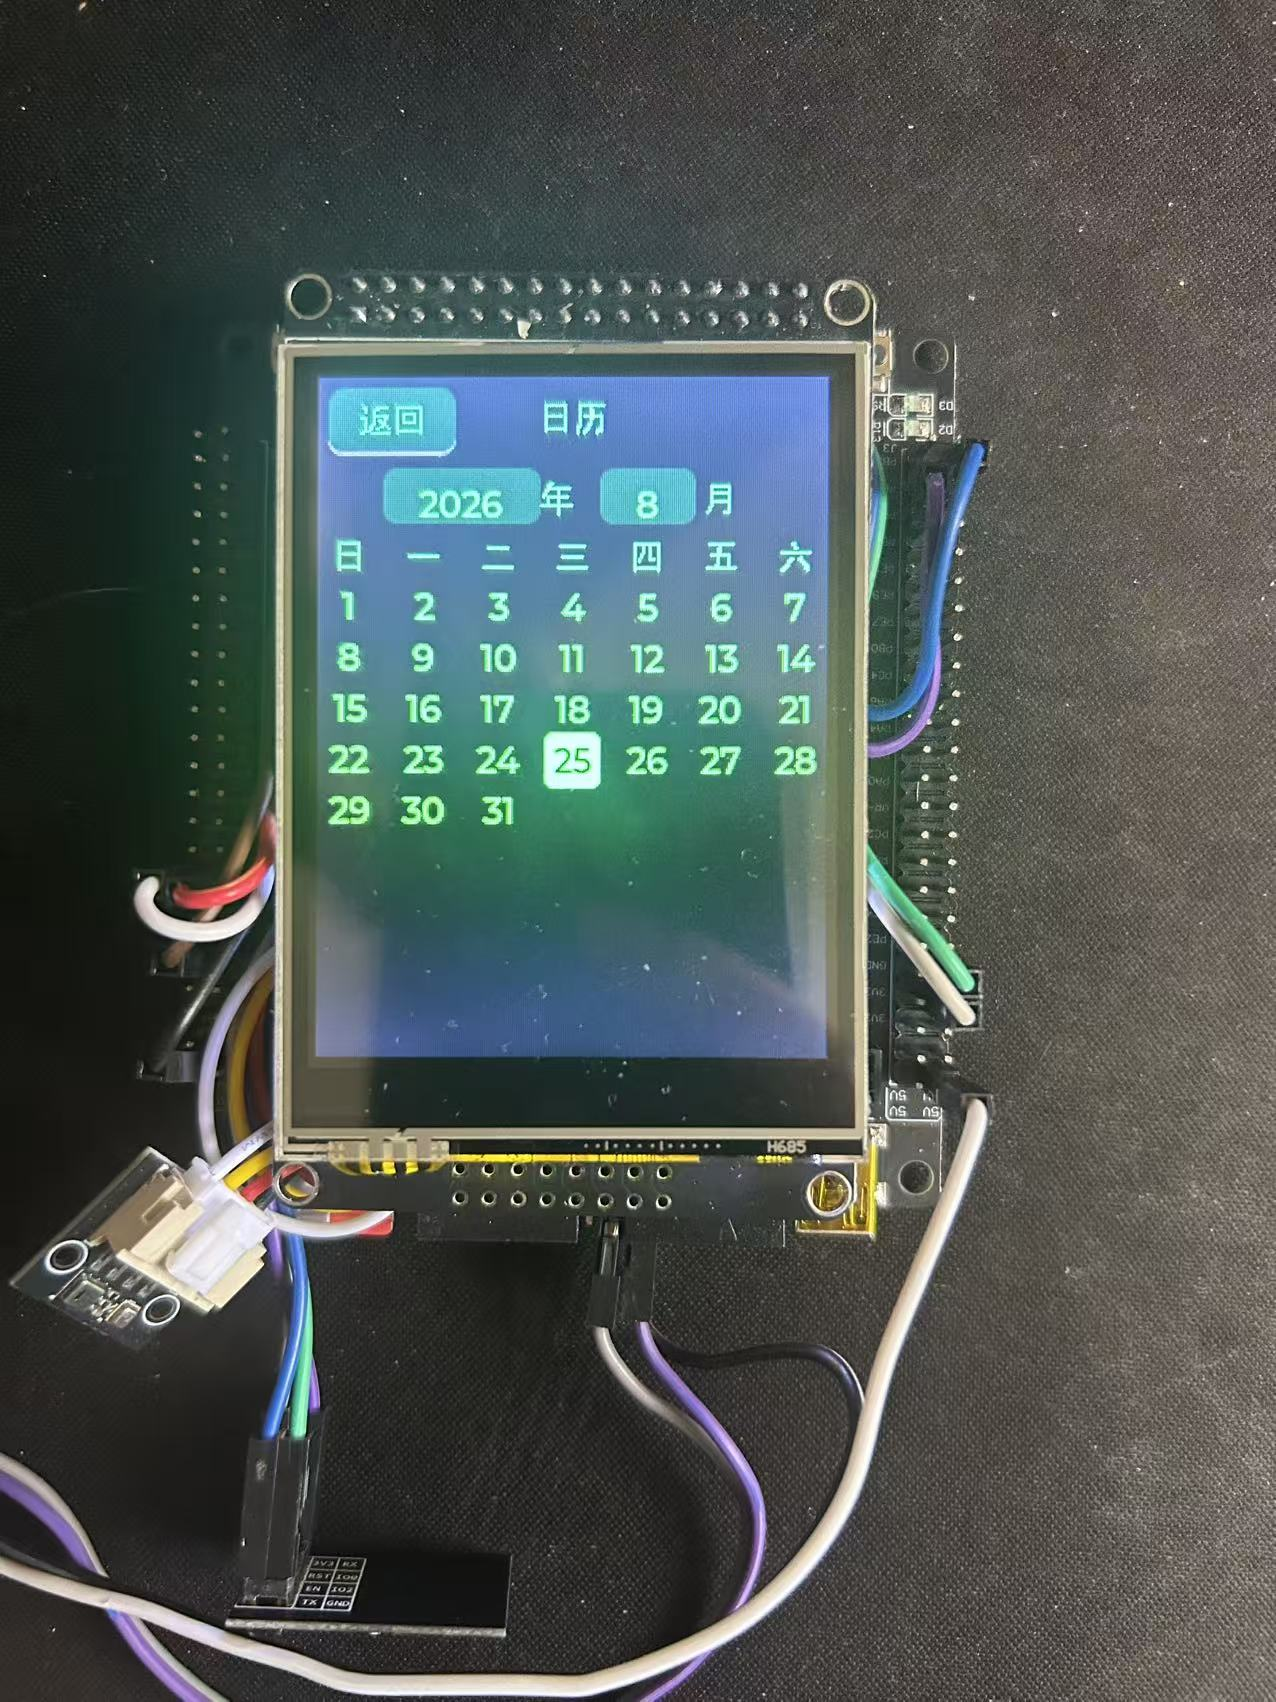
\includegraphics[width=0.42\textwidth]{日历.jpg}
\caption{模拟时钟与日历界面}
\end{figure}

\subsection{拼音输入法}

在 AI 对话页面实现了完整的拼音输入法，支持 GB2312 一级字库共 3755 个汉字：

\begin{itemize}
    \item 按拼音音节分组，405 个拼音码表，每组按使用频率排序候选字
    \item 6 个候选字按钮，实时匹配当前输入拼音串，支持左右翻页
    \item 支持模糊匹配（输入部分拼音即可显示候选字）
    \item 虚拟键盘输入，点击候选项自动替换末尾拼音串
    \item 常用汉字字库重新内置于 Flash，避免 SD 卡加载失败导致候选字显示为方框
\end{itemize}

\subsection{WiFi 选择与系统日志}

系统页面提供 WiFi 设置入口，WiFi 页面通过 ESP8266 的 \texttt{AT+CWLAP} 指令扫描周围热点，并将前 5 个 SSID 显示为可点击按钮。用户选择热点并输入密码后，STM32 通过 \texttt{AT+CWJAP} 指令控制 ESP8266 连接路由器；连接成功后，ESP8266 AT 固件会在自身 Flash 中保存 AP 信息。下次上电时，系统优先执行自动重连流程，不再占用 STM32 片内 Flash 存储 WiFi 配置。

系统状态页面由普通标签改为可滚动文本框，用于显示启动、联网、时钟同步、IAP 等调试信息。该设计避免状态信息增多时覆盖硬件信息，也便于在现场调试时回看历史日志。

\subsection{机器人面部表情动画}

系统实现了 4 种表情状态的状态机：

\begin{table}[H]
\centering
\begin{tabularx}{\textwidth}{llX}
\toprule
\textbf{状态} & \textbf{触发条件} & \textbf{动画效果} \\
\midrule
ROBOT\_IDLE & 默认状态、1.8秒无事件自动恢复 & 嘴部细线(80×5)闭合，眨眼(2-5秒随机)，眼球游走 \\
ROBOT\_LISTENING & 收到语音命令 & 嘴部微张(40×12)，提示正在聆听 \\
ROBOT\_THINKING & 提交AI请求 & 嘴部圆形(36×36)，表示思考中 \\
ROBOT\_SPEAKING & 收到AI回复 & 嘴部交替张合(60×36/60×8, 180ms周期)，模拟说话 \\
\bottomrule
\end{tabularx}
\caption{机器人表情状态}
\end{table}

表情动画的核心参数：

\begin{itemize}
    \item 眨眼：2--5 秒随机间隔，闭合 80ms，张开 120ms
    \item 眼球游走：1.2--2.8 秒随机间隔，移动范围 ±7px，过渡 300ms
    \item 说话：180ms 周期交替张合
    \item 自动恢复：无事件 1.8 秒后切回 IDLE
\end{itemize}

% ============================================================
\section{语音控制模块}
% ============================================================

\subsection{ASR PRO 离线语音识别}

ASR PRO 是天问（TWen51）平台的离线语音识别芯片，基于 CI-03T，支持约 200 条命令词，无需联网即可进行语音识别。

\subsubsection{硬件接线}

\begin{table}[H]
\centering
\begin{tabular}{lll}
\toprule
\textbf{ASR PRO} & \textbf{STM32F407} & \textbf{说明} \\
\midrule
TX (PA9)  & USART1 RX (PA10) & 串口交叉连接 \\
RX (PA10) & USART1 TX (PA9)  & 串口交叉连接 \\
GND       & GND              & 共地 \\
\bottomrule
\end{tabular}
\caption{ASR PRO 与 STM32 接线}
\end{table}

\subsubsection{通信协议}

ASR PRO 识别到命令词后，通过串口发送 ASCII 十进制数字 + 换行符：

\begin{lstlisting}
// ASR PRO 端代码（上位机 GUI 自动生成）
void ASR_CODE() {
  set_state_enter_wakeup(10000);
  switch (snid) {
   case 1: Serial.write('1'); break;  // 打开菜单
   case 2: Serial.write('2'); break;  // 待机画面
   case 3: Serial.write('3'); break;  // 系统状态
   case 4: Serial.write('4'); break;  // AI对话
   case 5: Serial.write('5'); break;  // 返回
   case 6: Serial.write('6'); break;  // 设置
   case 7: Serial.write('7'); break;  // 时钟
   case 8: Serial.write('8'); break;  // 日历
  }
  Serial.write('\n');
}
\end{lstlisting}

\subsubsection{STM32 端串口接收与解析}

STM32 通过 USART1 中断 + DMA 接收 ASR PRO 数据，实现了超时判帧机制：

\begin{itemize}
    \item 每收到一个字节，记录时间戳
    \item 收到换行符（0x0A）立即截帧
    \item 若 20ms 内无新字节且无换行符，自动截帧（兼容无换行符的 ASR 模块）
    \item 解析时遍历缓冲区，将 ASCII 十进制串转为整数 cmd\_id
    \item 解析完毕调用 \texttt{ASR\_FlushRx()} 清空缓冲区，重置 HAL 接收指针
\end{itemize}

% ============================================================
\section{环境传感器模块}
% ============================================================

\subsection{硬件组成与 I2C 总线}

环境监测部分由 AHT20 和 BMP280 两个 I2C 传感器组成。AHT20 负责温度、湿度采集，7 位器件地址为 \texttt{0x38}；BMP280 负责气压采集，并根据气压换算相对海拔，7 位器件地址为 \texttt{0x77}。二者共用传感器 I2C 总线，由 \texttt{sensorTask} 在启动时完成总线初始化、传感器初始化和周期采样。

\begin{table}[H]
\centering
\begin{tabularx}{\textwidth}{lllX}
\toprule
\textbf{器件} & \textbf{地址} & \textbf{采集量} & \textbf{用途} \\
\midrule
AHT20 & \texttt{0x38} & 温度、相对湿度 & 环境温湿度显示，提供舒适度参考 \\
BMP280 & \texttt{0x77} & 大气压强、相对海拔 & 环境气压显示，并换算海拔估计值 \\
\bottomrule
\end{tabularx}
\caption{环境传感器组成}
\end{table}

\subsection{AHT20 温湿度采集}

AHT20 初始化时需要等待芯片上电稳定，并检查校准使能位。程序向 AHT20 写入初始化命令后，若校准未完成则执行软复位并重试。采样时，STM32 发送触发测量命令，等待忙标志位 \texttt{0x80} 清零，再一次读取 6 字节数据帧。

AHT20 返回的湿度和温度均为 20 位原始值，程序在驱动层完成位拼接，在任务层按照数据手册公式换算为实际物理量：

\begin{align}
RH &= \frac{S_{RH}}{2^{20}} \times 100\% \\
T  &= \frac{S_T}{2^{20}} \times 200 - 50
\end{align}

其中 $S_{RH}$ 为湿度原始值，$S_T$ 为温度原始值。对应代码如下：

\begin{lstlisting}
uint32_t ct[2];
ATH20_Read_CTdata(ct);
data.temperature = (float)ct[1] * 200.0f / 1048576.0f - 50.0f;
data.humidity    = (float)ct[0] * 100.0f / 1048576.0f;
\end{lstlisting}

\subsection{BMP280 气压与海拔计算}

BMP280 的气压数据不能直接使用 ADC 原始值。初始化阶段，程序先从 \texttt{0x88} 起始地址读取 24 字节出厂校准参数，再配置温度 16 倍过采样、气压 8 倍过采样和 Normal 工作模式，同时打开 IIR 滤波配置。采样阶段从 \texttt{0xF7} 连续读取气压和温度原始数据，并使用芯片校准参数进行补偿计算。

补偿后的气压单位换算为 hPa，随后经过 5 点滤波，降低瞬时抖动。海拔值根据气压公式估算：

\begin{equation}
h = \frac{\left( \left(\frac{P_0}{P}\right)^{1/5.25588} - 1 \right) \times (25 + 273.15)}{0.0065}
\end{equation}

其中 $P$ 为当前气压，程序中参考气压 $P_0$ 取 \texttt{1015.7hPa}。该海拔值主要用于项目演示和环境变化趋势观察，若要获得绝对海拔，需要根据当地标准气压或实际海拔进行校准。

\subsection{FreeRTOS 数据流}

传感器采样被放在独立的 \texttt{sensorTask} 中，每 2 秒读取一次 AHT20 和 BMP280，并将四个浮点量打包为 \texttt{sensor\_data\_t} 结构体，通过 \texttt{sensor\_queue} 发送给 LVGL 任务。LVGL 任务只在当前页面为环境页面时取出队列数据并刷新标签，避免传感器采样阻塞界面刷新。

\begin{lstlisting}
typedef struct {
    float temperature;    /* AHT20 temperature */
    float humidity;       /* AHT20 humidity */
    float pressure;       /* BMP280 pressure */
    float altitude;       /* BMP280 altitude */
} sensor_data_t;

for (;;) {
    ATH20_Read_CTdata(ct);
    data.temperature = (float)ct[1] * 200.0f / 1048576.0f - 50.0f;
    data.humidity    = (float)ct[0] * 100.0f / 1048576.0f;

    BMP280GetData(&data.pressure, &bmp_temp, &data.altitude);
    osMessageQueuePut(sensor_queueHandle, &data, 0, 0);
    osDelay(2000);
}
\end{lstlisting}

这种设计将“采集”和“显示”解耦：传感器任务只负责稳定产生数据，界面任务只负责在合适的页面消费数据，从而降低 I2C 访问、浮点计算和 LVGL 刷新之间的相互影响。

\subsection{调试要点}

\begin{itemize}
    \item I2C 地址采用 7 位地址，驱动底层再根据读写方向生成总线地址，避免 \texttt{0x38}/\texttt{0x70} 混用
    \item AHT20 采样前检查忙标志位，防止测量未完成时读取到旧数据或无效数据
    \item BMP280 必须先读取出厂校准参数，否则气压补偿结果会明显异常
    \item 气压换算海拔受天气和当地参考气压影响，适合观察趋势，不宜作为高精度海拔计
    \item 传感器数据通过队列进入 UI，避免在 LVGL 刷新线程中直接执行阻塞式 I2C 访问
\end{itemize}

% ============================================================
\section{云端 AI 对话模块}
% ============================================================

\subsection{通信链路}

\begin{center}
STM32F407 $\xrightarrow{\text{USART3, 115200}}$ ESP8266 $\xrightarrow{\text{WiFi}}$ 路由器 $\xrightarrow{\text{Internet}}$ 阿里云 DashScope
\end{center}

ESP8266 运行 ESP-AT 固件，作为透传网卡，STM32 通过 AT 指令控制其完成 WiFi 连接和 HTTPS 请求。

\subsection{AT 指令序列}

\begin{table}[H]
\centering
\begin{tabularx}{\textwidth}{lX}
\toprule
\textbf{指令} & \textbf{作用} \\
\midrule
\texttt{AT}               & 自检，确认模块存活 \\
\texttt{ATE0}             & 关闭回显，避免数据污染 \\
\texttt{AT+CIPSERVER=0} / \texttt{AT+CIPMUX=0} & 退出 SoftAP 服务状态，恢复单连接 Station 模式 \\
\texttt{AT+CWMODE=1}      & 设置为 Station 模式 \\
\texttt{AT+CWLAP}         & 扫描周围 WiFi 热点，用于 WiFi 选择页面 \\
\texttt{AT+CWAUTOCONN=1}  & 允许 ESP8266 使用自身保存的 AP 信息自动重连 \\
\texttt{AT+CWJAP="ssid","pwd"} & 连接 WiFi 热点 \\
\texttt{AT+CIPSSLSIZE=4096}    & 调整 SSL 缓冲区大小 \\
\texttt{AT+CIPSSLCSNI="host"}  & 设置 SNI（Server Name Indication） \\
\texttt{AT+CIPSTART="SSL","host",443} & 建立 SSL 加密连接 \\
\texttt{AT+CIPSEND=<len>} & 申请发送 HTTP 请求 \\
$\cdots$ HTTP 请求体 $\cdots$ & 发送 JSON 格式的 API 请求 \\
\bottomrule
\end{tabularx}
\caption{ESP8266 AT 指令序列}
\end{table}

\subsection{HTTPS 通信的关键坑点}

\begin{enumerate}
    \item \textbf{SNI 必须设置}：阿里云 DashScope 走 CDN，同一 IP 对应多个域名。TLS 握手时 ESP8266 必须通过 \texttt{AT+CIPSSLCSNI} 告知服务器目标域名，否则服务器无法选择合适的证书，直接关闭连接。
    \item \textbf{确认 vs 响应}：\texttt{AT+CIPSEND} 的 ``Recv N bytes'' 是模块确认收到数据的字节数，不是远端响应。远端响应以 \texttt{+IPD} 开头。
    \item \textbf{超时设置}：大模型有冷启动延迟，首次请求可能超过 20 秒，接收超时需设为 60 秒。
    \item \textbf{响应解析}：HTTP 响应包含头部和 JSON body，需从 \texttt{"content"} 字段中提取 AI 回复文本，并处理 \texttt{\textbackslash n}、\texttt{\textbackslash "} 等转义字符。
\end{enumerate}

\subsection{API 调用}

调用阿里云 DashScope 兼容 OpenAI 格式的 Chat Completions API：

\begin{lstlisting}
POST https://dashscope.aliyuncs.com/compatible-mode/v1/chat/completions
Authorization: Bearer <API_KEY>
Content-Type: application/json

{
  "model": "qwen3.8-max",
  "messages": [
    {"role": "user", "content": "你好"},
    {"role": "assistant", "content": "你好！有什么可以帮助你的？"},
    {"role": "user", "content": "今天天气怎么样"}
  ]
}
\end{lstlisting}

系统维护最多 20 轮对话历史，每次请求将完整历史打包发送，实现多轮对话上下文。

% ============================================================
\section{Bootloader 与 IAP 固件升级}
% ============================================================

\subsection{Flash 启动布局}

系统采用 Bootloader + App 两段式启动结构：

\begin{lstlisting}[language=]
0x08000000 - 0x08007FFF   Bootloader
0x08008000 - 0x0807FFFF   App
\end{lstlisting}

上电后 CPU 首先从 \texttt{0x08000000} 运行 Bootloader。Bootloader 读取 App 起始地址处的初始栈指针和复位入口，判断 App 是否有效；若 App 有效且 PA0 下载键未按下，则设置 \texttt{VTOR} 和 \texttt{MSP} 后跳转到 App；若按下 PA0 或 App 无效，则进入 IAP 升级模式。

\subsection{串口 IAP 与 WiFi IAP}

IAP 升级包由 16 字节头部和 App 二进制载荷组成，头部包含 magic、版本号、镜像大小和 CRC32。Bootloader 在接收固件后执行三次校验：包头合法性、接收过程 CRC、写入 Flash 后读回 CRC。只有校验通过且 App 向量表合法，才认为升级成功。

系统支持两种升级通道：

\begin{itemize}
    \item \textbf{串口 IAP}：通过 USART1 与 PC 脚本握手，采用 \texttt{READY/NEXT} 分块发送机制。
    \item \textbf{WiFi IAP}：ESP8266 建立 SoftAP 和 TCP Server，PC 连接 \texttt{STM32-IAP} 热点后通过 TCP 发送升级包。
\end{itemize}

最终版本采用 PA0 作为下载键。正常上电时快速跳转 App，按住 PA0 上电时进入 IAP 等待，不再设置固定超时返回，方便现场升级和恢复。

% ============================================================
\section{关键代码模块}
% ============================================================

\subsection{项目文件结构}

\begin{lstlisting}[language=]
ai_project/
|-- Core/
|   |-- Inc/                    # 头文件
|   |   |-- FreeRTOSConfig.h    # FreeRTOS 配置
|   |   |-- ota_config.h         # Bootloader/App 地址与升级包配置
|   |   |-- pinyin_data.h       # 拼音输入法码表 (3755汉字)
|   |   |-- usart.h             # 串口配置
|   |   |-- fsmc.h              # FSMC 并口配置
|   |-- Src/
|       |-- main.c              # 入口，初始化外设
|       |-- freertos.c          # 核心：4个任务 + UI + 表情 + AI对话
|       |-- stm32f4xx_it.c      # 中断服务函数
|       |-- usart.c             # 串口初始化
|-- HARDWARE/
|   |-- ASR_PRO/
|   |   |-- asr_pro.c/h         # ASR PRO 串口驱动
|   |   |-- asrpro.txt          # ASR PRO 端代码参考
|   |-- ESP8266/
|   |   |-- esp8266.c/h         # ESP8266 AT 指令驱动
|   |-- LCD/
|   |   |-- lcd.c/h             # ILI9341 LCD 驱动
|   |-- LVGL/
|   |   |-- lv_port_disp.c/h    # LVGL 显示接口
|   |   |-- lv_port_indev.c/h   # LVGL 触摸输入接口
|   |-- ROBOT_FACE/
|   |   |-- robot_face_anim.c/h # 机器人表情动画
|   |-- aht20_bmp280/
|   |   |-- ATH20.c/h BMP280.c/h # 环境传感器驱动
|   |-- TOUCH/
|       |-- gt9147.c/h          # GT9147 触摸驱动
|       |-- touch.c/h           # 触摸抽象层
|-- Bootloader/                  # IAP 启动程序、升级协议与跳转逻辑
|-- Drivers/                    # STM32 HAL 库 + CMSIS
|-- tools/
|   |-- send_iap_update.ps1      # 串口 IAP 上位机脚本
|   |-- send_wifi_iap_update.ps1 # WiFi IAP 上位机脚本
|   |-- make_sd_update.ps1       # 生成带头部和 CRC 的 app.bin
|-- 项目图片/                    # 项目界面截图
|-- docs/                        # 报告、调试笔记与学习记录
\end{lstlisting}

\subsection{LVGL 显示接口}

\begin{lstlisting}
// lv_port_disp.c - 双缓冲，240×20 行刷新
static lv_color_t buf1[240 * 20];
static lv_color_t buf2[240 * 20];

static void disp_flush(lv_disp_drv_t *drv, const lv_area_t *area,
                       lv_color_t *color_p) {
    LCD_Color_Fill(area->x1, area->y1, area->x2, area->y2, (u16 *)color_p);
    lv_disp_flush_ready(drv);
}
\end{lstlisting}

\subsection{ASR PRO 串口帧解析}

\begin{lstlisting}
// asr_pro.c - 超时判帧 + ASCII 十进制解析
static int ASR_Parse(asr_msg_t *msg) {
    if (!asr.data_ready || asr.rx_len == 0) return 0;

    uint32_t id = 0;
    for (int i = 0; i < asr.rx_len; i++) {
        uint8_t c = asr.rx_buf[i];
        if (c >= '0' && c <= '9')
            id = id * 10 + (c - '0');
        else
            break;
    }

    if (id == 0 || id > 160) { ASR_FlushRx(); return 0; }
    msg->cmd_id = (uint8_t)id;
    ASR_FlushRx();  // 重置缓冲区，重新开始接收
    return 1;
}
\end{lstlisting}

\subsection{任务间消息队列通信}

\begin{lstlisting}
// freertos.c - lvglTask 主循环 (简化)
for (;;) {
    // 1. 读取 ESP8266 状态消息，更新状态页面
    while (osMessageQueueGet(esp_rx_queueHandle, &m, NULL, 0) == osOK) { ... }

    // 2. 读取 AI 回复，追加到对话历史
    if (osMessageQueueGet(esp_ai_queueHandle, ai_buf, NULL, 0) == osOK) {
        chat_add_message("assistant", ai_buf);
        robot_face_set_state(ROBOT_SPEAKING);  // 触发说话表情
    }

    // 3. 读取 ASR 语音命令，切换页面
    if (osMessageQueueGet(asr_queueHandle, &asr_msg, NULL, 0) == osOK) {
        robot_face_set_state(ROBOT_LISTENING);
        switch (asr_msg.cmd_id) {
            case ASR_CMD_IDLE:  lv_scr_load(idle_scr); break;
            case ASR_CMD_MAIN_MENU: lv_scr_load(main_scr); break;
            // ... 其他页面切换
        }
    }

    // 4. 表情自动恢复：1.8秒无事件 → IDLE
    robot_face_tick();
    lv_timer_handler();
    osDelay(5);
}
\end{lstlisting}

% ============================================================
\section{调试与问题解决}
% ============================================================

\subsection{ASR PRO 串口通信问题}

\textbf{问题}：ASR PRO 语音命令无法切换 STM32 屏幕页面。

\textbf{根因}：ASR\_Parse 解析完一帧数据后仅将 \texttt{data\_ready} 置 0，未重置 \texttt{rx\_len} 和 HAL 接收指针。导致：
\begin{itemize}
    \item \texttt{rx\_len} 持续累积增长
    \item \texttt{HAL\_UART\_Receive\_IT} 指针越跑越偏，新数据存不到 \texttt{buf[0]}
    \item 解析器始终读取 \texttt{buf[0]} 的旧数据，同一命令被无限重复解析
\end{itemize}

\textbf{解决}：在 \texttt{ASR\_Parse} 末尾调用 \texttt{ASR\_FlushRx()}，一次性重置所有状态：\texttt{rx\_len=0}、清空缓冲区、\texttt{HAL\_UART\_Receive\_IT} 重新指向 \texttt{buf[0]}。

\subsection{ESP8266 HTTPS 连接问题}

详见 \texttt{DEBUG.md}，核心问题与解决方案：
\begin{itemize}
    \item \textbf{SNI 缺失}：ESP8266 老版本固件不支持 SNI，导致 TLS 握手失败，服务器直接关闭连接。通过在 \texttt{AT+CIPSTART} 前调用 \texttt{AT+CIPSSLCSNI} 解决。
    \item \textbf{确认误判}：将 \texttt{AT+CIPSEND} 的确认信息误判为远端响应，导致解析逻辑错误。
    \item \textbf{冷启动超时}：大模型首次调用需加载模型，超时从 20 秒调整为 60 秒。
\end{itemize}

\subsection{IAP 与 Flash 空间问题}

\textbf{问题}：在增加 Bootloader/IAP 后，需要同时解决 App 起始地址、向量表跳转、升级包校验和 Flash 空间不足问题。

\textbf{解决}：将 Bootloader 固定在 \texttt{0x08000000--0x08007FFF}，App 固定从 \texttt{0x08008000} 链接运行；升级包通过脚本添加头部与 CRC32；Bootloader 跳转 App 前设置 \texttt{VTOR} 与 MSP，并在跳转前重新使能中断。最终 App 使用完整剩余 Flash 空间，常用汉字字库重新内置于 Flash，保证 AI 输入候选字稳定显示。

\subsection{SD 卡字库与 WiFi 配置取舍}

\textbf{问题}：为节省 Flash 曾尝试将常用汉字字库放入 SD 卡，但 SD 卡初始化、挂载和文件读取链路较长，容易导致字库加载失败，从而出现 AI 输入候选字显示方框。

\textbf{解决}：最终将常用 3000 多字字库放回 Flash，保证显示稳定；WiFi 配置不再占用 STM32 Flash，而是利用 ESP8266 AT 固件自身保存 AP 信息与自动重连能力，实现手动配置一次后自动联网。


% ============================================================
\section{技术指标}
% ============================================================

\begin{table}[H]
\centering
\begin{tabularx}{\textwidth}{lX}
\toprule
\textbf{指标} & \textbf{参数} \\
\midrule
CPU 主频 & 168MHz, Cortex-M4 \\
RAM 使用 & 约 1.16MB ZI 数据，主要使用外部 SRAM 扩展内存池与 LVGL 缓冲 \\
Flash 使用 & App 镜像约 460KB / 480KB 可用 App 区，含常用汉字字库与拼音码表 \\
LCD 刷新率 & 约 30--50 FPS (LVGL 双缓冲) \\
ASR 识别延迟 & < 500ms (离线) \\
环境采集 & AHT20 温湿度 + BMP280 气压/海拔，2 秒周期刷新 \\
AI 对话延迟 & 3--20 秒 (取决于网络和模型负载，已加入超时与文本过滤处理) \\
串口波特率 & 115200 (USART1 接 ASR PRO, USART3 接 ESP8266) \\
WiFi 标准 & 802.11 b/g/n, 2.4GHz \\
固件升级 & Bootloader + 串口 IAP + WiFi IAP，App 起始地址 0x08008000 \\
\bottomrule
\end{tabularx}
\caption{系统技术指标}
\end{table}

% ============================================================
\section{总结与展望}
% ============================================================

\subsection{项目成果}

本项目成功实现了一款集语音控制、虚拟表情动画、环境监测、模拟时钟、日历与云端 AI 对话于一体的智能交互终端。主要成果包括：

\begin{enumerate}
    \item 基于 FreeRTOS 的多任务系统架构，任务间通过消息队列解耦，模块化程度高
    \item 基于 LVGL 的图形界面，包含 6 个页面，支持拼音输入法（3755 汉字）
    \item 机器人面部表情动画系统，4 种状态自动切换，具有情感化表达
    \item ASR PRO 离线语音命令控制，支持 8 条页面切换命令
    \item AHT20/BMP280 环境监测模块，支持温度、湿度、气压和海拔数据采集显示
    \item ESP8266 通过 HTTPS 连接阿里云 DashScope，实现多轮 AI 对话
    \item 实现 Bootloader、串口 IAP 与 WiFi IAP，支持按键进入升级模式和固件 CRC 校验
    \item 实现 WiFi 扫描选择、ESP8266 自动重连、可滚动系统日志和 Flash 内置常用汉字字库
\end{enumerate}

\subsection{未来优化方向}

\begin{enumerate}
    \item \textbf{语音输入升级}：将 ASR PRO 扩展为全双工语音对话，或替换为 ESP32-S3 实现云端流式语音识别
    \item \textbf{表情丰富化}：增加更多表情状态（开心、难过、惊讶、困惑），添加眉毛/腮红等面部元素
    \item \textbf{传感器扩展}：在现有 AHT20/BMP280 基础上继续加入光照、人体感应、空气质量等传感器，扩展环境感知能力
    \item \textbf{物联网功能}：通过 WiFi 获取天气、新闻、课程表等信息，扩展实用功能
    \item \textbf{升级体验优化}：在 App 内加入版本号显示、升级进度展示与失败回滚策略
\end{enumerate}

\end{document}
